\chapter{VCO}
\label{ch:VCO}
\section{Allgemeines}

Oszillatorschaltung:

\begin{figure}[h]
	\centering
	\setlength{\fboxsep}{1pt} %Abstand der Linien zur Abbildung
	\setlength{\fboxrule}{1pt} %Dicke der Linie
	\fbox{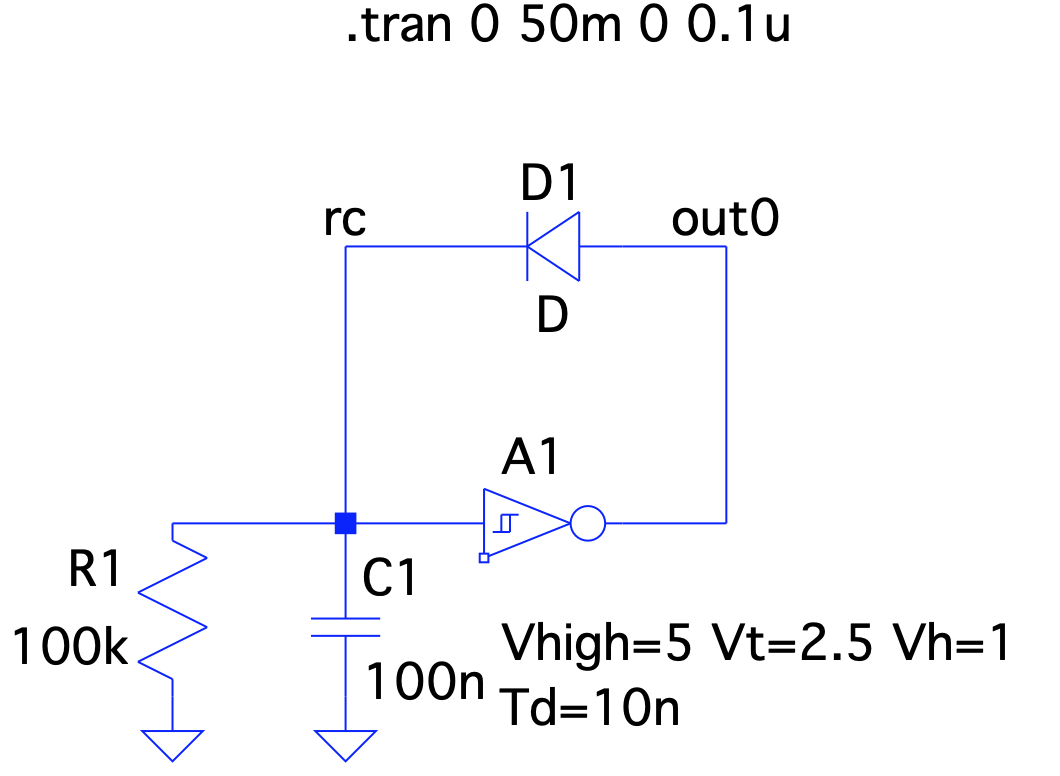
\includegraphics[width=0.8\textwidth]{figures/Oszillator_Schaltbild}}
	\caption{Oszillatorschaltung}
	\label{fig:fig:Oszillatorschaltung}
\end{figure}

Um die Oszillatorschaltung, die den Kern des VCOs darstellt, zu verstehen, erfolgt im Folgenden die Betrachtung des Punkts \textit{rc}.
Zu Beginn messen wir überhaupt keine Spannung, weil der Kondensator leer ist und noch nichts durch unsere Diode fließt. 
Das bedeutet, dass am Ausgang des Schmitt-Triggers eine Spannung anliegt, da wir unter dem unteren Eingangsschwellenwert liegen. 
Jetzt haben wir einen Stromfluss vom Ausgang über die Diode zu unserem zentralen Punkt. 
Da der Kondensator zunächst leer ist, fließt der ganze Strom in diesen hinein.
Während sich der Kondensator auflädt, steigt die Spannung an unserem zentralen Punkt rapide an.
Dieser Spannungsanstieg wird aber auch vom Schmitt-Trigger-Eingang registriert - als Reaktion darauf fällt der Ausgang auf 0 V ab, sobald der Kondensator aufgeladen ist und die Spannung die obere Eingangsschwelle überschreitet.
Das bedeutet, dass kein zusätzlicher Strom durch die Diode fließt und sich der Kondensator wieder entlädt. 
Aber weil der Widerstand die Strommenge begrenzt, die durchfließen kann, wird sich unser Kondensator nicht sofort entladen. 
Auf dem Spannungsdiagramm sehen wir also einen langsamen Abfall. 
Das geht so lange, bis wir den unteren Schwellenwert unseres Schmitt-Trigger-Inverters erreichen. 
Sobald wir diese Schwelle auf dem Weg nach unten überschritten haben, beginnt der Zyklus von neuem - denn jetzt schwingt der Ausgang wieder nach oben, und alles wiederholt sich.

Der entstandene Signalverlauf stellt eine  Sägezahnschwingung dar.

\begin{figure}[htbp]
	\centering
	\setlength{\fboxsep}{1pt} %Abstand der Linien zur Abbildung
	\setlength{\fboxrule}{1pt} %Dicke der Linie
	\fbox{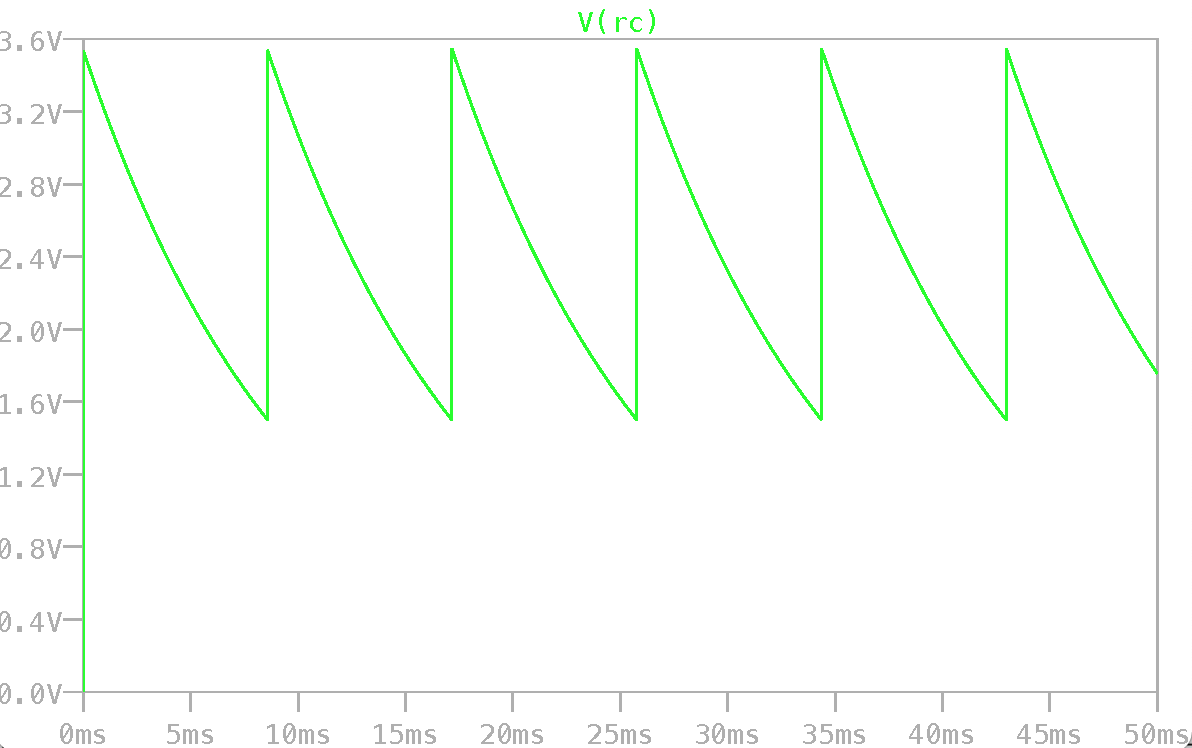
\includegraphics[width=0.8\textwidth]{figures/Oszillator_Signalverlauf}}
	\caption{Oszillator Signalverlauf}
	\label{fig:fig:Oszillator_Signalverlauf}
\end{figure}

\section{Schaltplan}
bla bla bla

\section{Platine}
bla bla bla

\section{Mechanischer Aufbau}
bla bla bla